\documentclass[a4paper]{report}

% Polish letters packages (for OS X)
\usepackage[utf8]{inputenc}
\usepackage{polski}
\usepackage[polish]{babel}

\usepackage[T1]{fontenc}
\usepackage{textcomp}
\usepackage{lmodern}
\usepackage[a4paper, margin=1in]{geometry}
% do robienia tabel które mieszczą się na stronie (łamanie linii w kolumnach tabeli)
\usepackage{tabulary}
% do wrzucania obrazów
\usepackage{graphicx}
% scieżka do folderu z plikami graficznymi
\graphicspath{{./images/}}
% do opisu tabel i rysunków
\usepackage{caption}
\captionsetup[table]{name=Tabela}
% do tabel żeby robić kreski (toprule, bottomrule itp)
\usepackage{booktabs}
% do kolorowania wierszy w tabeli
\usepackage{color, colortbl}
\definecolor{Gray}{gray}{0.75}
% do tworzenia własnych styli formatowania komórek tabel
\usepackage{array}
\newcolumntype{X}[1]{>{\raggedright\let\newline\\\arraybackslash\hspace{0pt}}m{#1}}
% do schowania napisu rozdzial n
\usepackage{titlesec} 
\titleformat{\chapter}[display]{\normalfont\bfseries}{}{0pt}{\Huge}

\title{\huge Układy Cyfrowe i Systemy Wbudowane 2\\Projekt Synthesia}
\date{} % pusta data
\author{Jan Luch\hspace{42pt} 218150  \\Dawid Aksamski\hspace{5pt} 218429}


\begin{document}

\frenchspacing
\pagenumbering{gobble}
\maketitle
\newpage

\tableofcontents
\newpage

\pagenumbering{arabic}

\chapter{Wstęp}
	\section{Cel i zakres}
	\section{Sprzęt}
	\section{Protokoły}
	\section{Interfejsy}
	\section{Algorytmy}

\chapter{Projekt}
	\section{Hierarchia}
	Krótka proza
		\subsection{Schemat}
		\subsection{Submoduły}
		
\chapter{Moduły}
	\section{Generator Dźwięku}
		\subsection{Symbol}
		\subsection{Porty}
		\subsection{Najważniejsze sygnały i procesy}
		\subsection{FSM}
		Graf i opis kodu
		\subsection{Symulacja}
	\section{Sterownik VGA}
		\subsection{Symbol}
			\begin{figure}[h!]
				\centering
				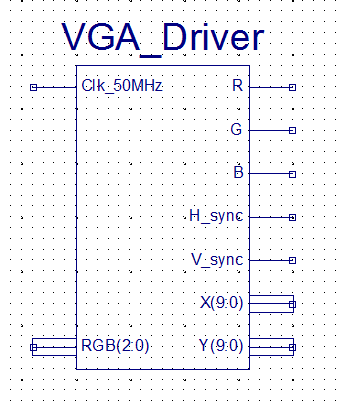
\includegraphics{vgadriver2.png}
				\caption{Moduł sterujący wyjciem VGA}
			\end{figure}
		\subsection{Porty}
		\subsection{Najważniejsze sygnały i procesy}
		\subsection{FSM}
		Graf i opis kodu
		\subsection{Symulacja}
	\section{Przełącznik}
		\subsection{Symbol}
			\begin{figure}[h!]
				\centering
				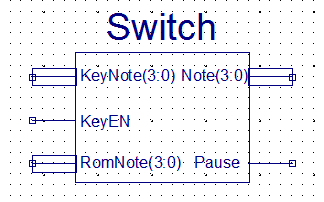
\includegraphics{switch2.png}
				\caption{Moduł Switch}
			\end{figure}
		\subsection{Porty}
		\subsection{Najważniejsze sygnały i procesy}
		\subsection{FSM}
		Graf i opis kodu
		\subsection{Symulacja}
	\section{Czytnik kodów z klawiatury}
		\subsection{Symbol}
			\begin{figure}[h!]
				\centering
				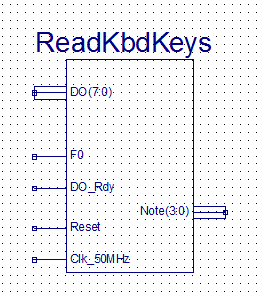
\includegraphics{readkbdkeys2.png}
				\caption{Moduł czytający kody z klawiatury}
			\end{figure}
		\subsection{Porty}
		\subsection{Najważniejsze sygnały i procesy}
		\subsection{FSM}
		Graf i opis kodu
		\subsection{Symulacja}
	\section{Synthesia}
		\subsection{Symbol}
		\subsection{Porty}
		\subsection{Najważniejsze sygnały i procesy}
		\subsection{FSM}
		Graf i opis kodu
		\subsection{Symulacja}
	
\chapter{Implementacja}
	\section{Rozmiar}
	LUT, BRAM
	\section{fmax}
	\section{Podręcznik użytkowania urządzenia}
	(Zdjęcia)
	
\chapter{Podsumowanie}
	\section{Ocena krytyczna}	
	\section{Kierunki dalszych prac}
	
\chapter{Literatura}

\begin{figure}
	\caption{Sample figure}
\end{figure}
		
\begin{table}
	\caption{Sample table}
\end{table}

% Compile twice to generate list of tables and figures properly
\begin{appendix}
	\listoffigures
	\listoftables
\end{appendix}



\end{document}
